\documentclass{article}

\usepackage[utf8]{inputenc}
\usepackage[T1]{fontenc}
\usepackage{amsmath,amssymb}
\usepackage{textcomp}
\usepackage{float}
\usepackage{listings}
\usepackage{hyperref}
\usepackage{graphicx}
\usepackage[table]{xcolor}
\usepackage{todonotes}
\usepackage{tikz}
\usepackage{pgf-umlcd}
\usetikzlibrary{positioning, fit, calc, shapes, arrows, er}

\definecolor{codegreen}{rgb}{0,0.6,0}
\definecolor{codepurple}{rgb}{0.58,0,0.82}
\definecolor{codegray}{rgb}{0.5,0.5,0.5}

\lstdefinelanguage{math}{
  keywords={var, let, in, end},
  sensitive=false,
  comment=[l]{//},
  morecomment=[s]{/*}{*/},
  morestring=[b]',
  morestring=[b]",
}

\lstdefinelanguage{xtend}{
  keywords={override, void, if, return, public, static, new, val, def, retrun, int, switch, throw},
  sensitive=false,
  comment=[l]{//},
  morecomment=[s]{/*}{*/},
  morestring=[b]',
  morestring=[b]",
}

\lstdefinestyle{wstyle}{
    keywordstyle=\color{codepurple},
    stringstyle=\color{codegreen},
    commentstyle=\color{codegray},
}

\lstset{style=wstyle}

\begin{document}

\title{Assingment 2 - External DSL Interpreter}
\author{Marc Bertelsen\\
\textbf{berte20@student.sdu.dk}}

\maketitle

\pagebreak

\section{Desing}
\todo{design}
% how to structure a math expression
% has to fit the syntax of the existing tests 

\subsection{Metamodel}
\todo{metamodel}

% Expression
% Presidence of operations: mult - div -> add - sub

% EXPR
%   left (operation right)?
%   left could be product or quotient (mult or div)
%   left could be sum or difference (plus or minus)
%   left could be constant

\todo{redo}
\begin{figure}[H]
    \centering
    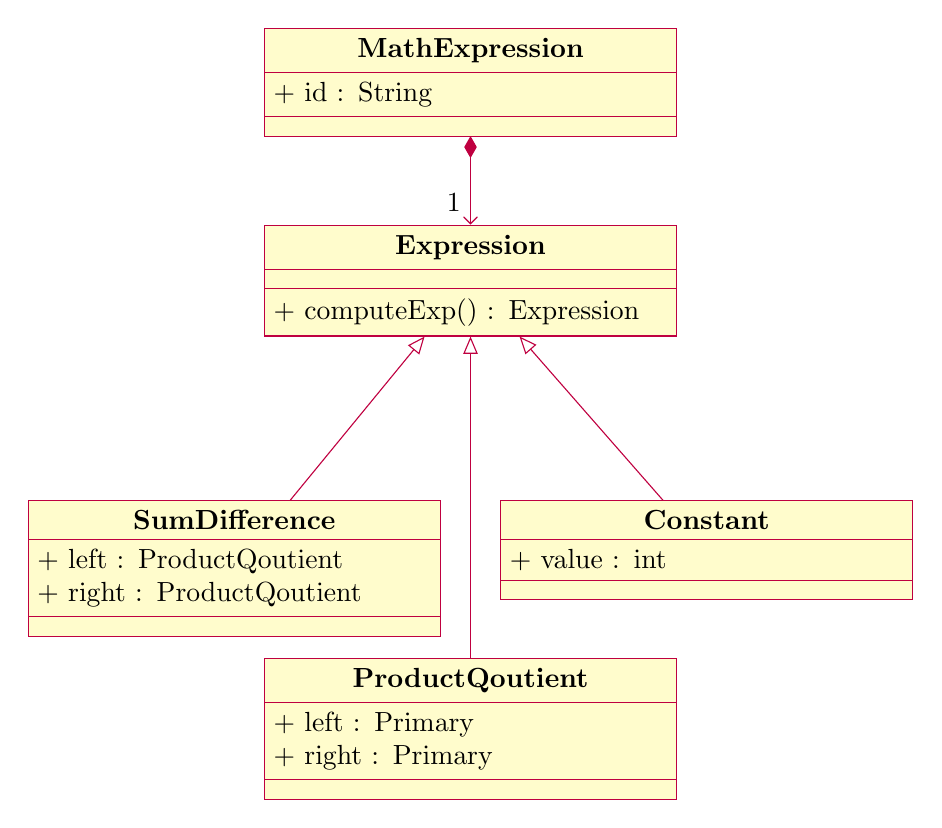
\begin{tikzpicture}
        \begin{class}{MathExpression}{0,0}{
            \attribute{+ id : String}
        }
        \end{class}
        \begin{class}{Expression}{0,-2.5}{
            \operation{+ computeExp() : Expression}
        }
        \end{class}
        \begin{class}{SumDifference}{-3,-6}{
            \attribute{+ left : ProductQoutient}
            \attribute{+ right : ProductQoutient}
        }
        \inherit{Expression}
        \end{class}
        \begin{class}{ProductQoutient}{0,-8}{
            \attribute{+ left : Primary}
            \attribute{+ right : Primary}
        }
        \inherit{Expression}
        \end{class}
        \begin{class}{Constant}{3,-6}{
            \attribute{+ value : int}
        }
        \inherit{Expression}
        \end{class}
        \composition{MathExpression}{}{1}{Expression}
    \end{tikzpicture}
    \caption{Mathematical Expression Metamodel}
\end{figure}
    

\subsection{Syntax}

% number

% equation
% var ref
% var binding
\begin{center}
    \begin{lstlisting}[language={math}, captionpos={b}, caption={Examples of *.math syntax}]
        var a = 1
        var b = 1 + 1
        var c = a + b
        var d = let x = 1 + 1 in a end
    \end{lstlisting}
\end{center}

\section{Implmentation}

\subsection{XText syntax}
\begin{lstlisting}[caption={XText syntax}, captionpos={b}]
grammar dk.sdu.mmmi.mdsd.Math with org.eclipse.xtext.common.Terminals

generate math "http://www.sdu.dk/mmmi/mdsd/Math"

MathExp:
    exps+=Exp*
;

Exp:
    'var' name=ID '=' exp=SumDiff
;

SumDiff returns Expression:
    ProdQuot (('+'{Add.left=current} | '-'{Sub.left=current}) right=ProdQuot)*
;

ProdQuot returns Expression:
    Primary (('*'{Mul.left=current} | '/'{Div.left=current}) right=Primary)*
;

Primary returns Expression:
    Constant | Parenthesis | VariableUse | VariableBinding
;

Parenthesis returns Expression:
    {Parenthesis} '(' exp=SumDiff ')'
;

Constant returns Expression:
    {Constant} value=INT
;

VariableUse returns Expression:
    {VariableUse} ref=ID
;

VariableBinding returns Expression:
    {VariableBinding} 'let' id=ID '=' binding=SumDiff 'in' body=SumDiff 'end'
;
\end{lstlisting}

\subsection{XTend Generator}
% just the computation code
\begin{lstlisting}[language={xtend}, caption={XTend generator}, captionpos={b}]
override void doGenerate(
    Resource resource, IFileSystemAccess2 fsa, IGeneratorContext context) {
    val variables = resource.allContents.filter(MathExp).next.compute
    
    // You can replace with hovering, see Bettini Chapter 8
    variables.displayPanel
}

def static Map<String, Integer> compute(MathExp math) {
    val variables = new HashMap<String, Integer>()
    
    val tmp = new HashMap<String, Expression>()
    math.exps.forEach[exp | tmp.put(exp.name, exp.exp)]
    
    math.exps.forEach[exp | {
        val res = exp.exp.computeExp(variables, tmp)			
        variables.put(exp.name, res)
    }]
    return variables
}

def static int computeExp(
    Expression exp, Map<String, Integer> vars, Map<String, Expression> tmp) {
    switch exp {
        Add: exp.left.computeExp(vars, tmp)+exp.right.computeExp(vars, tmp)
        Sub: exp.left.computeExp(vars, tmp)-exp.right.computeExp(vars, tmp)
        Mul: exp.left.computeExp(vars, tmp)*exp.right.computeExp(vars, tmp)
        Div: exp.left.computeExp(vars, tmp)/exp.right.computeExp(vars, tmp)
        Constant: exp.value
        Parenthesis: exp.exp.computeExp(vars, tmp)
        VariableUse:
        {
            if (!vars.keySet.contains(exp.ref)) {
                val res = tmp.get(exp.ref).computeExp(vars, tmp)
                vars.put(exp.ref, res)
            }
            vars.get(exp.ref)
        }
        VariableBinding: exp.body.computeExp(
            vars.bind(exp.id, exp.binding.computeExp(vars, tmp)), tmp)
        default: throw new Error("Could not compute expression")
    }
}

def static Map<String, Integer> bind(
    Map<String, Integer> vars, String key, Integer value) {
    val binding = new HashMap<String, Integer>(vars)
    binding.put(key, value)
    binding
}
\end{lstlisting}

\subsection{XTend Validator}
\begin{lstlisting}[language={xtend}, caption={XTend validator}, captionpos={b}]
public static val DUBLICATE_VAR = 'dublicateVar'

val set = new HashSet<String>()

@Check
def clearSet(MathExp m) {
    set.clear
}

@Check
def checkNoDublicateVar(Exp exp) {
    if (set.contains(exp.name)) {
        warning("var " + exp.name + " has already been declared",
            MathPackage.Literals.EXP__NAME,
            DUBLICATE_VAR
        )
        return
    }
    set.add(exp.name)
}
\end{lstlisting}
\section{Test}
\todo{test results}
% if i can get it to work :)

Current implmentation passes \textbf{MathExampleTest}, \textbf{MathParsingTest}, and \textbf{MathValidatorTest}, but failes \textbf{MathScopeTest}.

\begin{figure}[H]
    \centering
    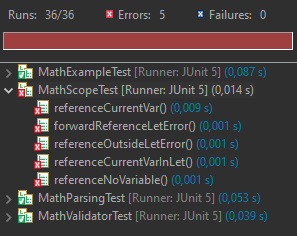
\includegraphics{tests.PNG}
\end{figure}

\section{Conclusion}
\todo{conclusion}
% using 

\end{document}